% -----------------------------------------------------------------------------
% NeuroWork — Avance 2  (plantilla oficial Springer LNCS)
% Compilar en Overleaf: subir este archivo + la carpeta figs/ y usar pdfLaTeX.
% Clase llncs (ya disponible en Overleaf; no requiere instalar nada).
% -----------------------------------------------------------------------------
\documentclass[runningheads]{llncs}

\usepackage[T1]{fontenc}
\usepackage[utf8]{inputenc}
\usepackage{graphicx}
\usepackage{booktabs}
\usepackage{url}
\graphicspath{{figs/}}

\begin{document}

\title{NeuroWork: asistente inteligente para la búsqueda y adaptación laboral de personas neurodivergentes mediante inteligencia artificial generativa y minería de datos}

\author{Yahir Ortega Ramos}
\institute{Instituto Tecnológico de Tijuana, Tijuana, Baja California, México\\
\email{L21212578@tectijuana.edu.mx}}

\maketitle

\begin{abstract}
Este documento reporta el avance del proyecto NeuroWork, una aplicación web (PWA) de apoyo
a la búsqueda de empleo para personas neurodivergentes. En esta etapa el sistema pasó de
propuesta a un \textbf{prototipo funcional} con once módulos operativos, integración de
inteligencia artificial generativa mediante un proxy seguro y una \textbf{base de datos
relacional} (SQLite) conectada a la aplicación. Se incorporó un conjunto de \textbf{41
pruebas automáticas} que verifican la analítica, la generación de currículums, la base de
datos y la API del servidor. La validación con personas usuarias se planifica para la fase
final. El avance global estimado es de aproximadamente 85\,\%.

\keywords{neurodivergencia \and búsqueda de empleo \and inteligencia artificial generativa \and minería de datos \and SQLite \and accesibilidad.}
\end{abstract}

\noindent Repositorio: \url{https://github.com/yahirortegasistemas-bit/-neurowork}

\section{Desarrollo funcional parcial}
El sistema se encuentra en una \textbf{fase operativa inicial estable}. La aplicación
contempla once módulos, todos navegables y funcionales (Tabla~\ref{tab:modulos}).

\begin{table}[htbp]
\caption{Módulos del sistema y su estado.}
\label{tab:modulos}
\centering
\small
\begin{tabular}{lll}
\toprule
Módulo & Estado & Función principal\\
\midrule
Panel & Funcional & Resumen del día: perfil, checklist, objetivos, dificultad\\
Progreso & Funcional & Minería de datos y gráficas de avance\\
Perfil & Funcional & Datos de contacto, experiencia y formación\\
Habilidades & Funcional & Registro con categoría y nivel de confianza (1--5)\\
CV & Funcional & Generación/adaptación con IA y cuatro plantillas\\
Entrevistas & Funcional & Vacante, simulador, preparación y respuestas\\
Reuniones & Funcional & Instrucciones convertidas en pasos\\
Checklist & Funcional & Tareas con repetición diaria\\
Objetivos & Funcional & Metas con porcentaje de avance\\
Preferencias & Funcional & Modalidad, horario y ajustes razonables\\
Privacidad & Funcional & Transparencia sobre el manejo de datos\\
\bottomrule
\end{tabular}
\end{table}

\textbf{Funcionalidad destacada (CV).} Genera un borrador con IA a partir del perfil, permite
adaptarlo a una vacante concreta y descargarlo en un documento \texttt{.doc} con cuatro
diseños profesionales (\emph{Moderno}, \emph{Ejecutivo}, \emph{Clásico} y \emph{Minimalista}),
con vista previa antes de descargar y fechas alineadas a la derecha.

\textbf{Sobre el inicio de sesión.} NeuroWork \textbf{no implementa autenticación} de forma
deliberada. Su modelo es \emph{local-first}: la información permanece en el equipo de la
persona y no existe un servidor de cuentas en la nube. Añadir un \emph{login} obligaría a
almacenar datos personales en un servidor, lo que contradiría el principio de minimización.
Esta decisión puede revisarse si el proyecto requiere operación multiusuario.

\section{Prototipo funcional / versión de prueba}
El prototipo es \textbf{ejecutable y navegable}, e instalable como aplicación (PWA).
\textbf{Requisitos:} Node.js 22+ y un navegador moderno. \textbf{Ejecución:}
\texttt{node server/server.js} y abrir \texttt{http://127.0.0.1:8787}.

\noindent\textbf{Flujo principal demostrable:}
\begin{enumerate}
\item Registrar perfil y habilidades.
\item Generar un CV con IA y descargarlo en cualquiera de los cuatro diseños.
\item Adaptar el CV a una vacante pegada por la persona.
\item Practicar un simulacro de entrevista con retroalimentación por respuesta.
\item Registrar objetivos y checklist; observar el progreso en gráficas.
\item Comprobar el respaldo en la base de datos (\texttt{/api/db}).
\end{enumerate}
La aplicación funciona \textbf{sin conexión} para todo lo local mediante un \emph{Service
Worker}; solo las funciones de IA requieren red.

\section{Avance de la base de datos y arquitectura}
\subsection{Decisión y estado}
Se integró una base de datos \textbf{relacional SQLite} usando el módulo nativo
\texttt{node:sqlite} (sin dependencias externas). El archivo reside en
\texttt{server/data/neurowork.db}, en el propio equipo, y está excluido del repositorio.
\textbf{Estado:} diseñada e implementada parcialmente; queda pendiente la migración de datos
antiguos y la sincronización multiusuario.

\subsection{Esquema (23 tablas con relaciones)}
\begin{verbatim}
workspace (raíz)
 |-1:1- profile            |-1:N- experiences        |-1:N- skills
 |-1:1- preferences        |-1:N- education          |-1:N- languages
 |-1:1- prep_plans         |-1:N- certifications     |-1:N- projects
 |-1:1- vacancy_analyses   |-1:N- cv_documents -N:1- cv_templates
 |-1:N- checklist_items    |-1:N- goals              |-1:N- activity_log
 |-1:N- snapshots          |-1:N- prepared_answers   |-1:N- professional_links
 |-1:N- meetings -1:N- meeting_steps
 '-1:N- interview_sessions -1:N- interview_questions
\end{verbatim}
Cada tabla tiene clave primaria; las tablas hijas referencian \texttt{workspace(id)} con
\texttt{ON DELETE CASCADE}. El DDL completo está en \texttt{server/db.js}.

\subsection{Conexión con la aplicación}
La persistencia es doble y transparente: \textbf{localStorage siempre} y, si el servidor
está activo, \textbf{respaldo en SQLite}. Si no hay servidor, la app sigue funcionando igual.
La clave de API nunca viaja al navegador: se inyecta en el servidor desde
\texttt{server/.env} (Tabla~\ref{tab:api}).

\begin{table}[htbp]
\caption{Endpoints de la API.}
\label{tab:api}
\centering
\small
\begin{tabular}{lll}
\toprule
Método & Endpoint & Función\\
\midrule
PUT & \texttt{/api/state} & Guarda el estado (llamado por \texttt{saveState()})\\
GET & \texttt{/api/state} & Recupera el estado si no había datos locales\\
DELETE & \texttt{/api/state} & Borra el respaldo («Reiniciar datos»)\\
GET & \texttt{/api/db} & Motor, ruta y conteo de filas por tabla\\
\bottomrule
\end{tabular}
\end{table}

\section{Evidencias del avance}
Las siguientes capturas corresponden al prototipo en ejecución con \textbf{datos de ejemplo},
tomadas automáticamente con un navegador en modo sin interfaz.

\begin{figure}[htbp]
\centering
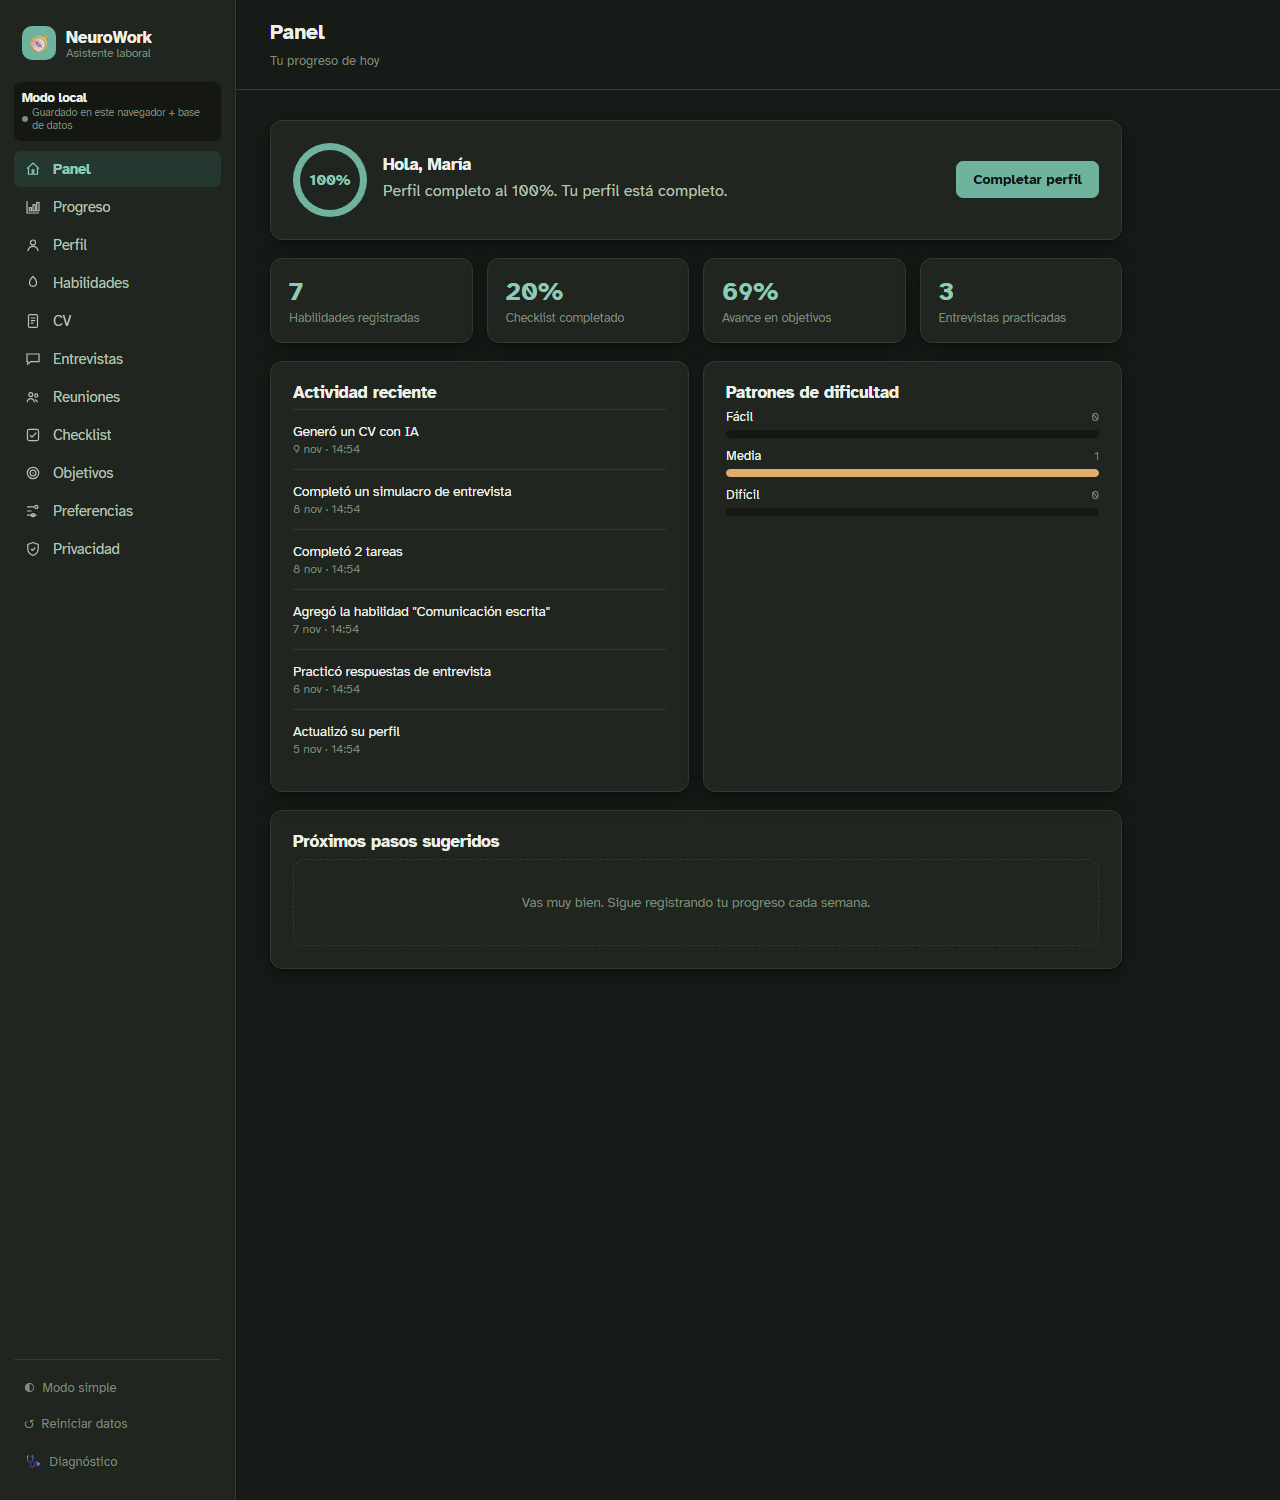
\includegraphics[width=\textwidth]{01-panel.png}
\caption{Panel principal: resumen del progreso del día, actividad reciente y patrones de dificultad.}
\end{figure}

\begin{figure}[htbp]
\centering
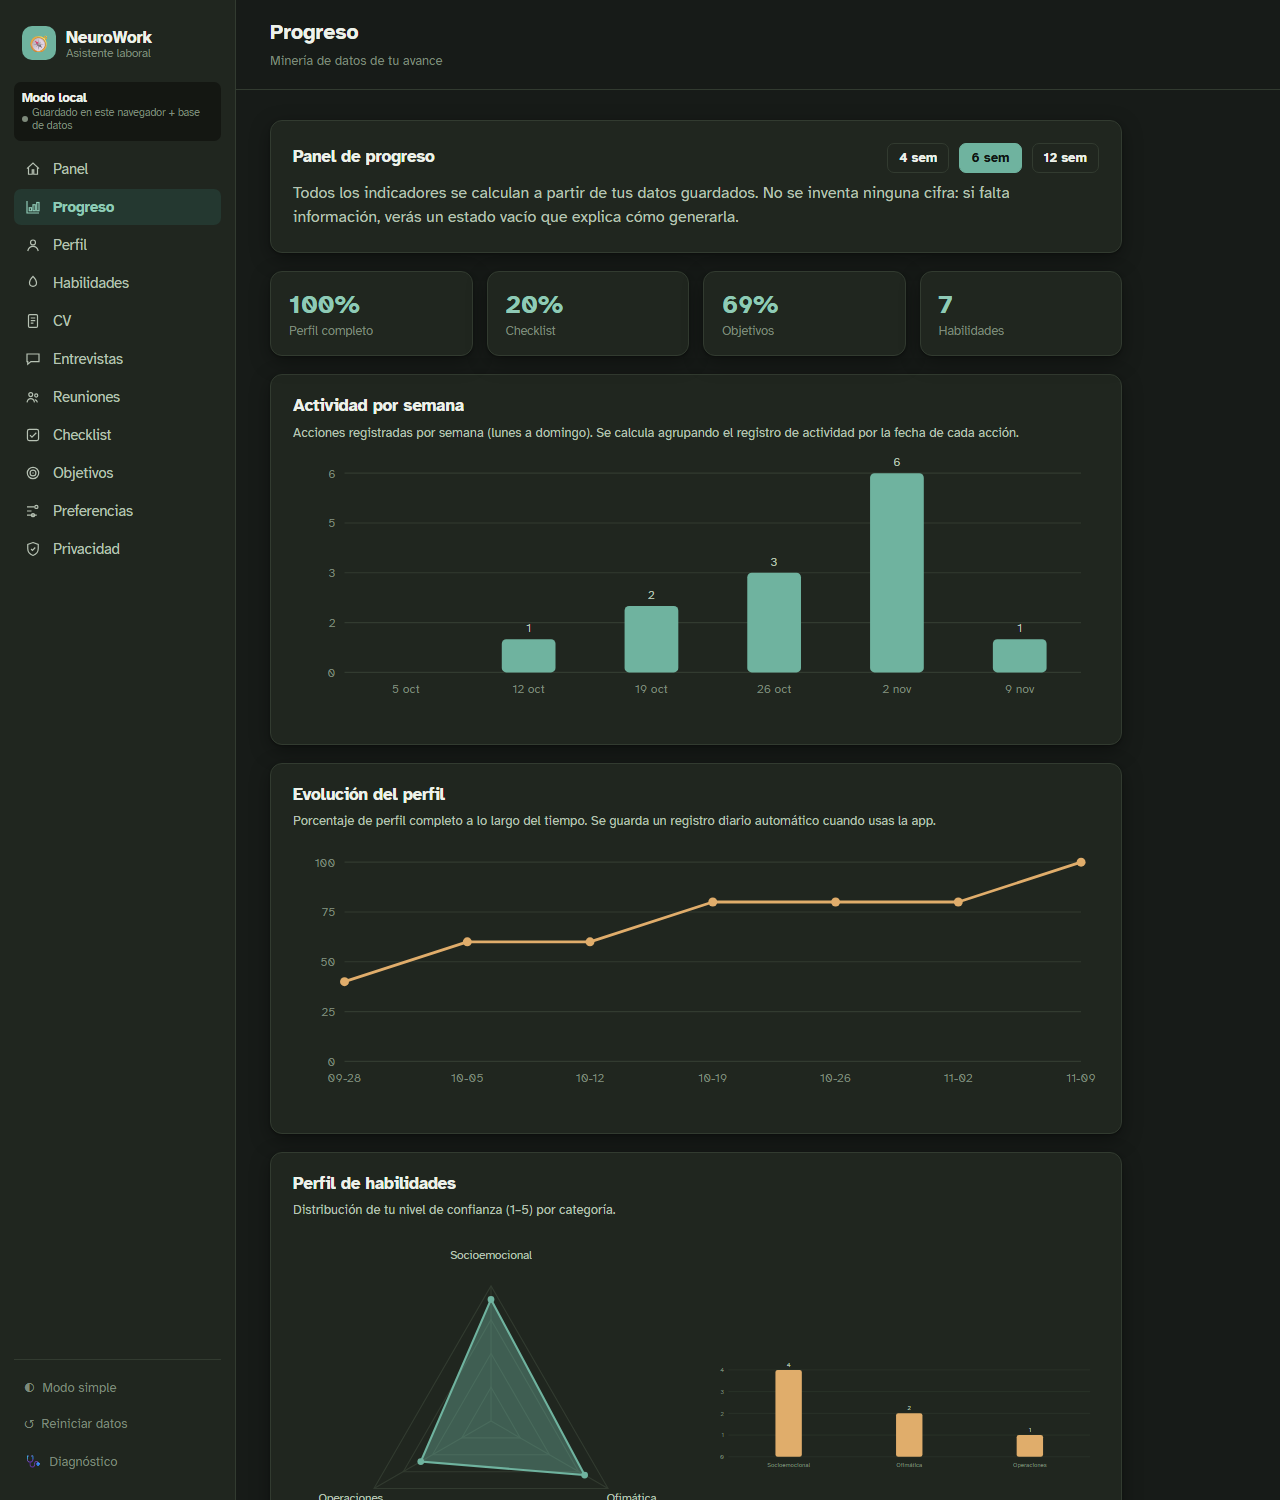
\includegraphics[width=\textwidth]{02-progreso.png}
\caption{Módulo de minería de datos: actividad semanal, evolución del perfil y perfil de habilidades.}
\end{figure}

\begin{figure}[htbp]
\centering
\begin{minipage}{0.49\textwidth}\centering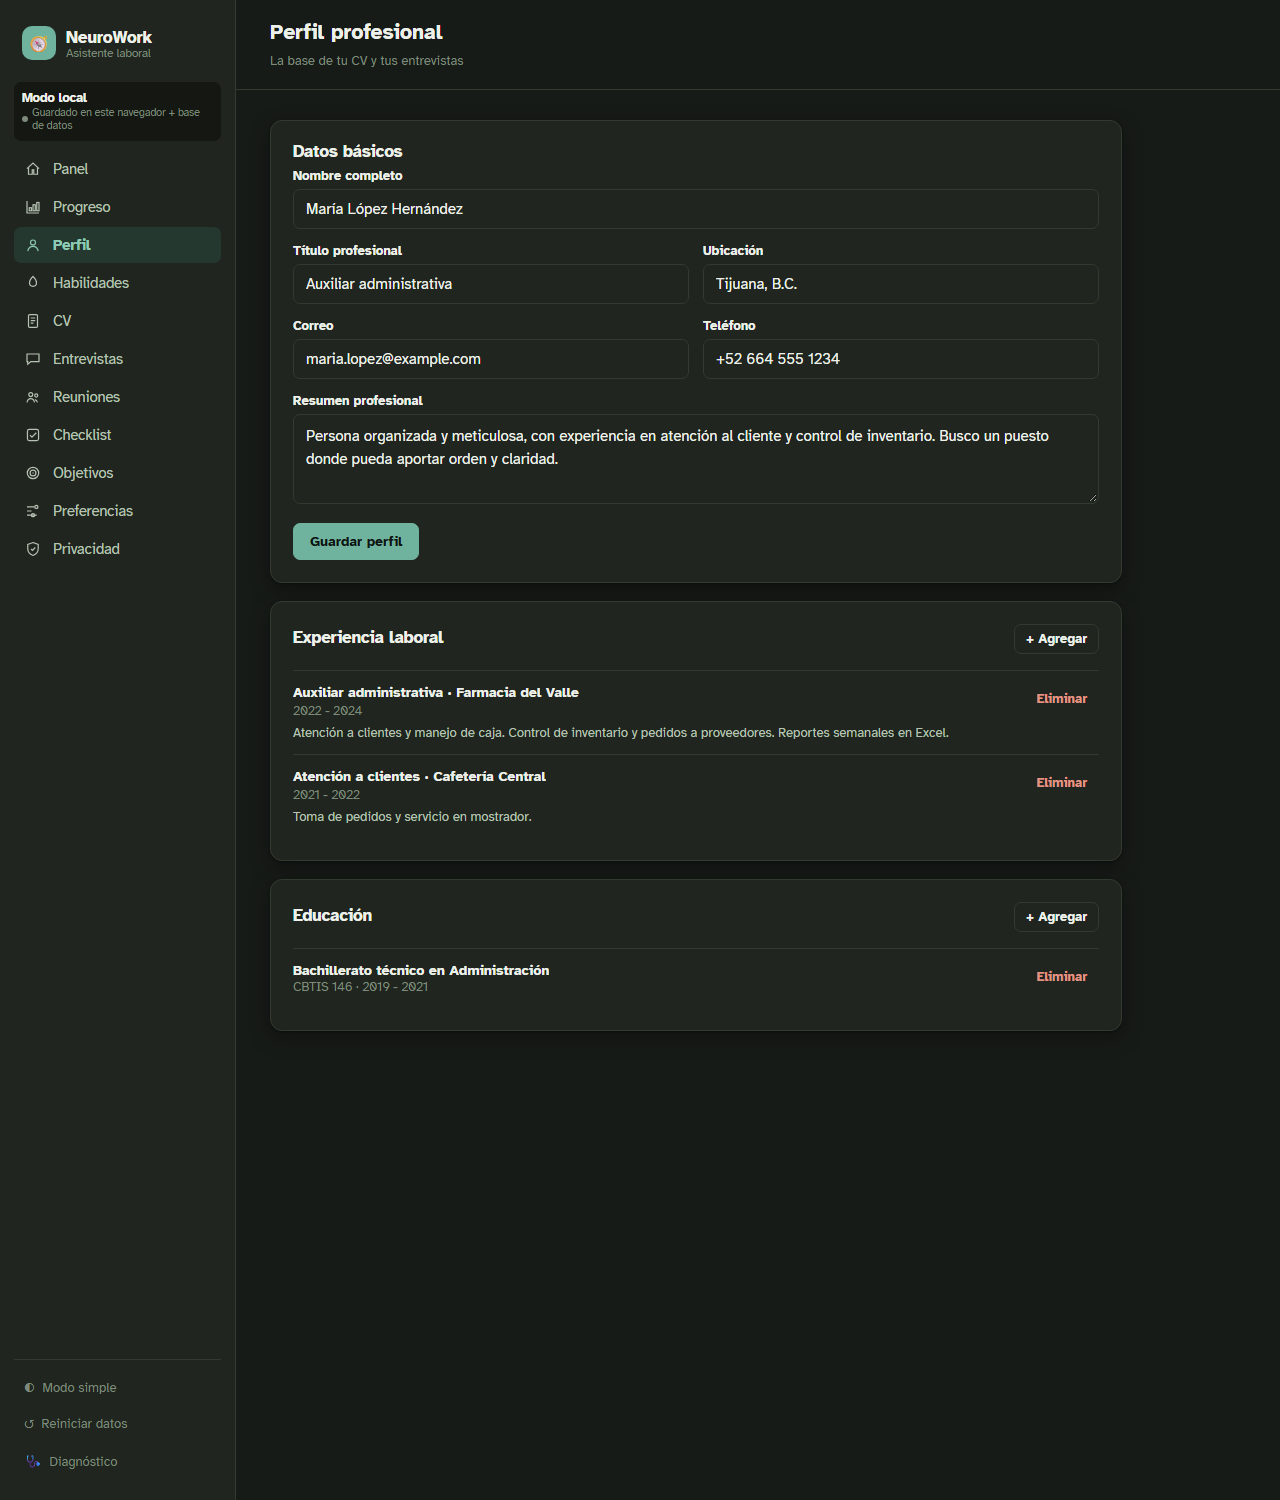
\includegraphics[width=\linewidth]{03-perfil.png}\end{minipage}\hfill
\begin{minipage}{0.49\textwidth}\centering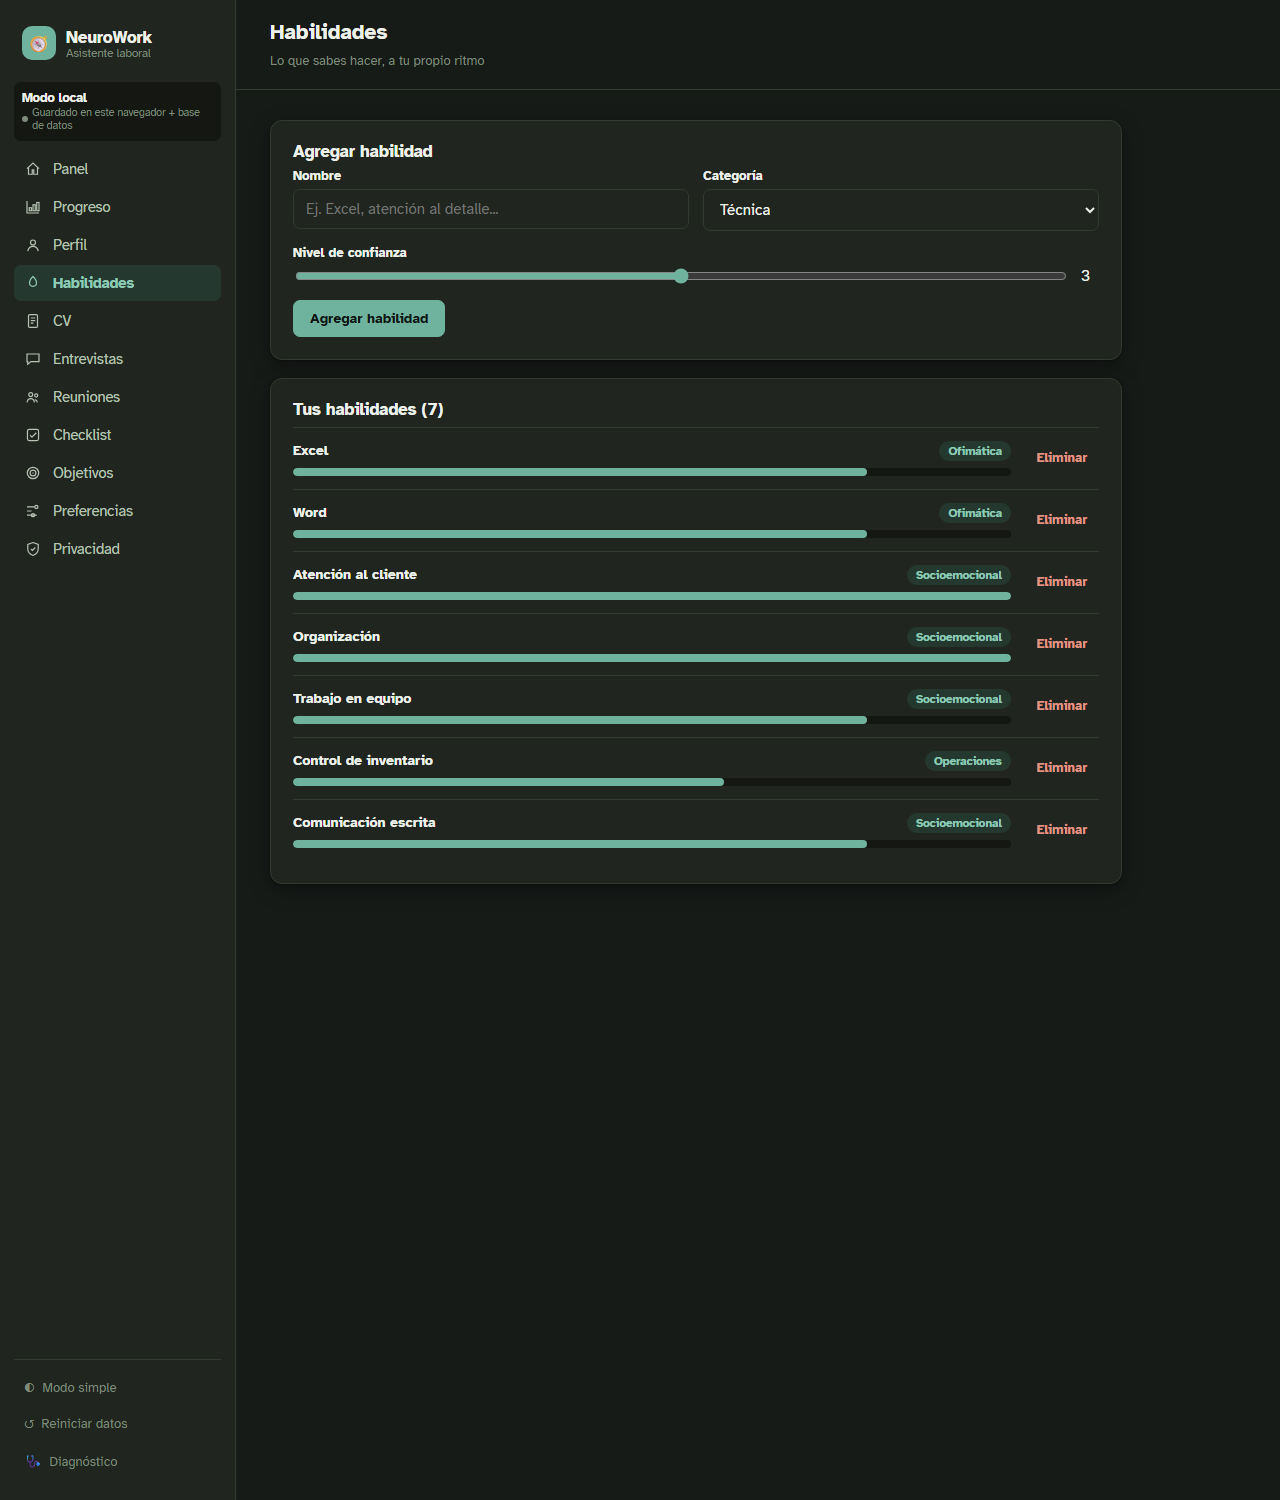
\includegraphics[width=\linewidth]{04-habilidades.png}\end{minipage}
\caption{Izquierda: perfil profesional. Derecha: registro de habilidades con nivel de confianza (1--5).}
\end{figure}

\begin{figure}[htbp]
\centering
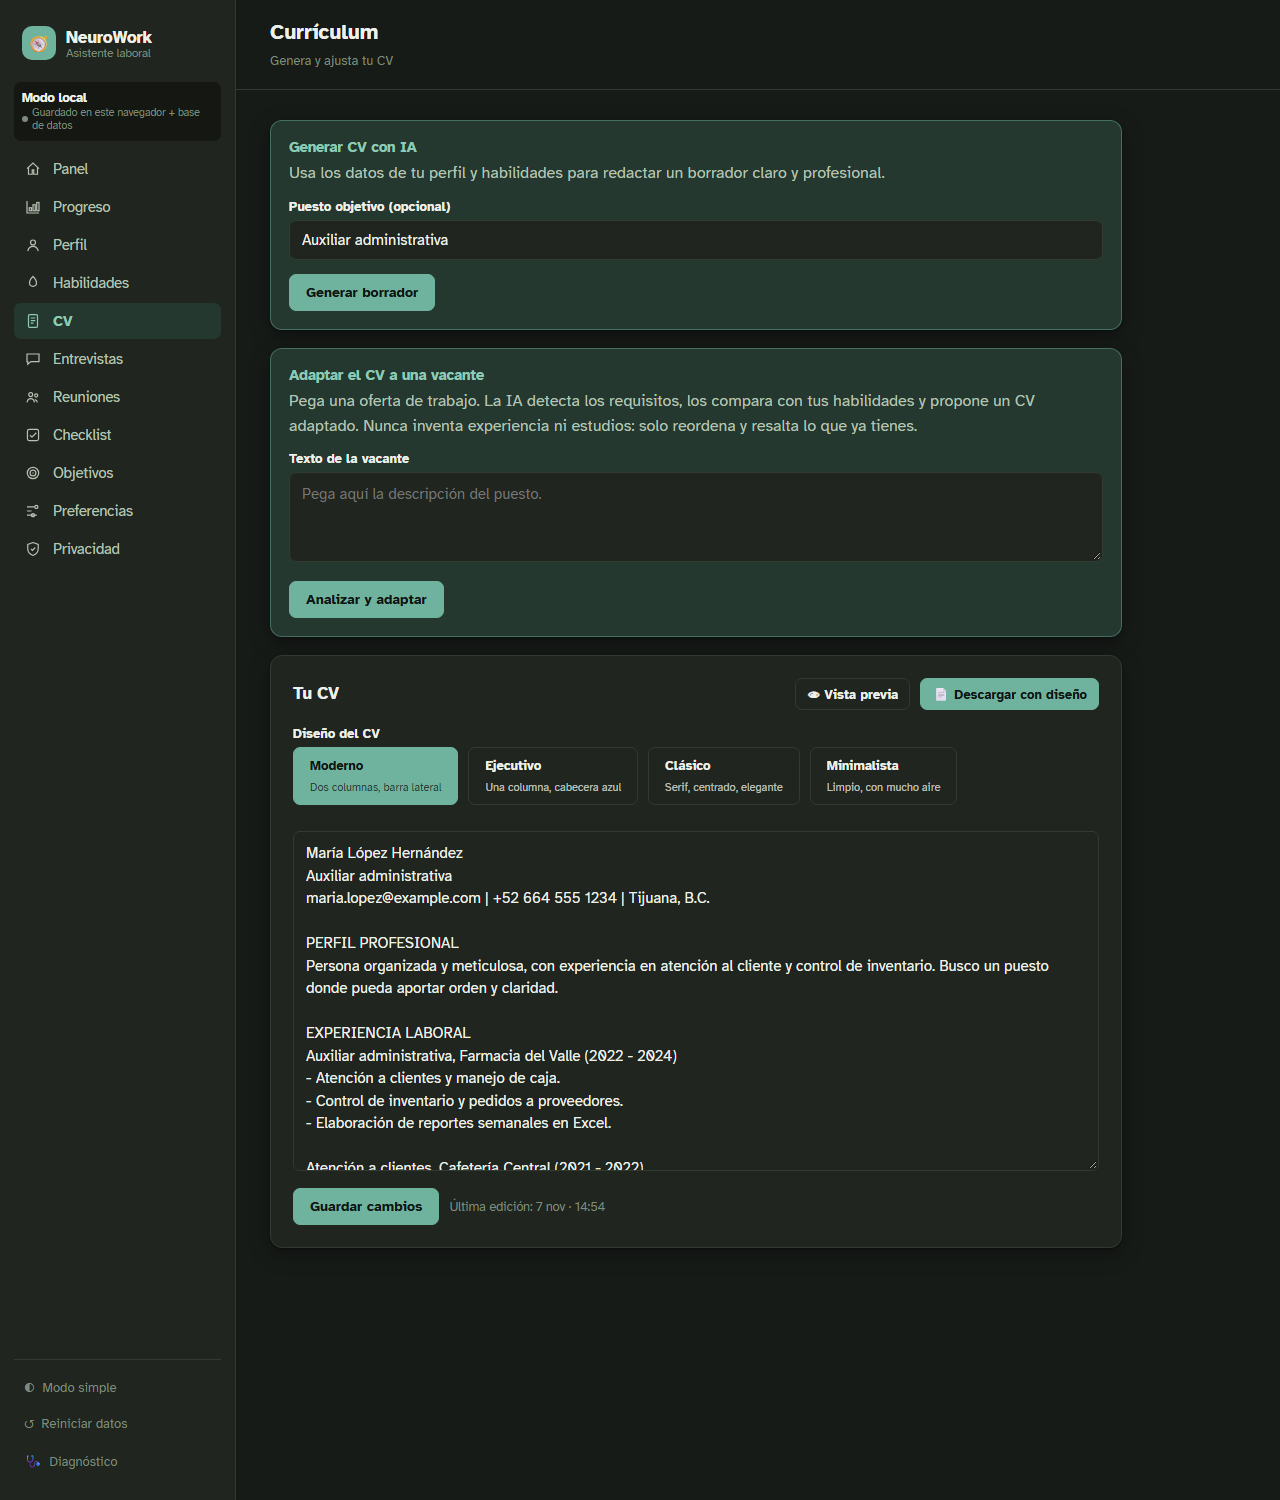
\includegraphics[width=\textwidth]{05-cv.png}
\caption{Módulo de CV: generación asistida por IA, adaptación a una vacante, selector de diseños, vista previa y descarga.}
\end{figure}

\begin{figure}[htbp]
\centering
\begin{minipage}{0.49\textwidth}\centering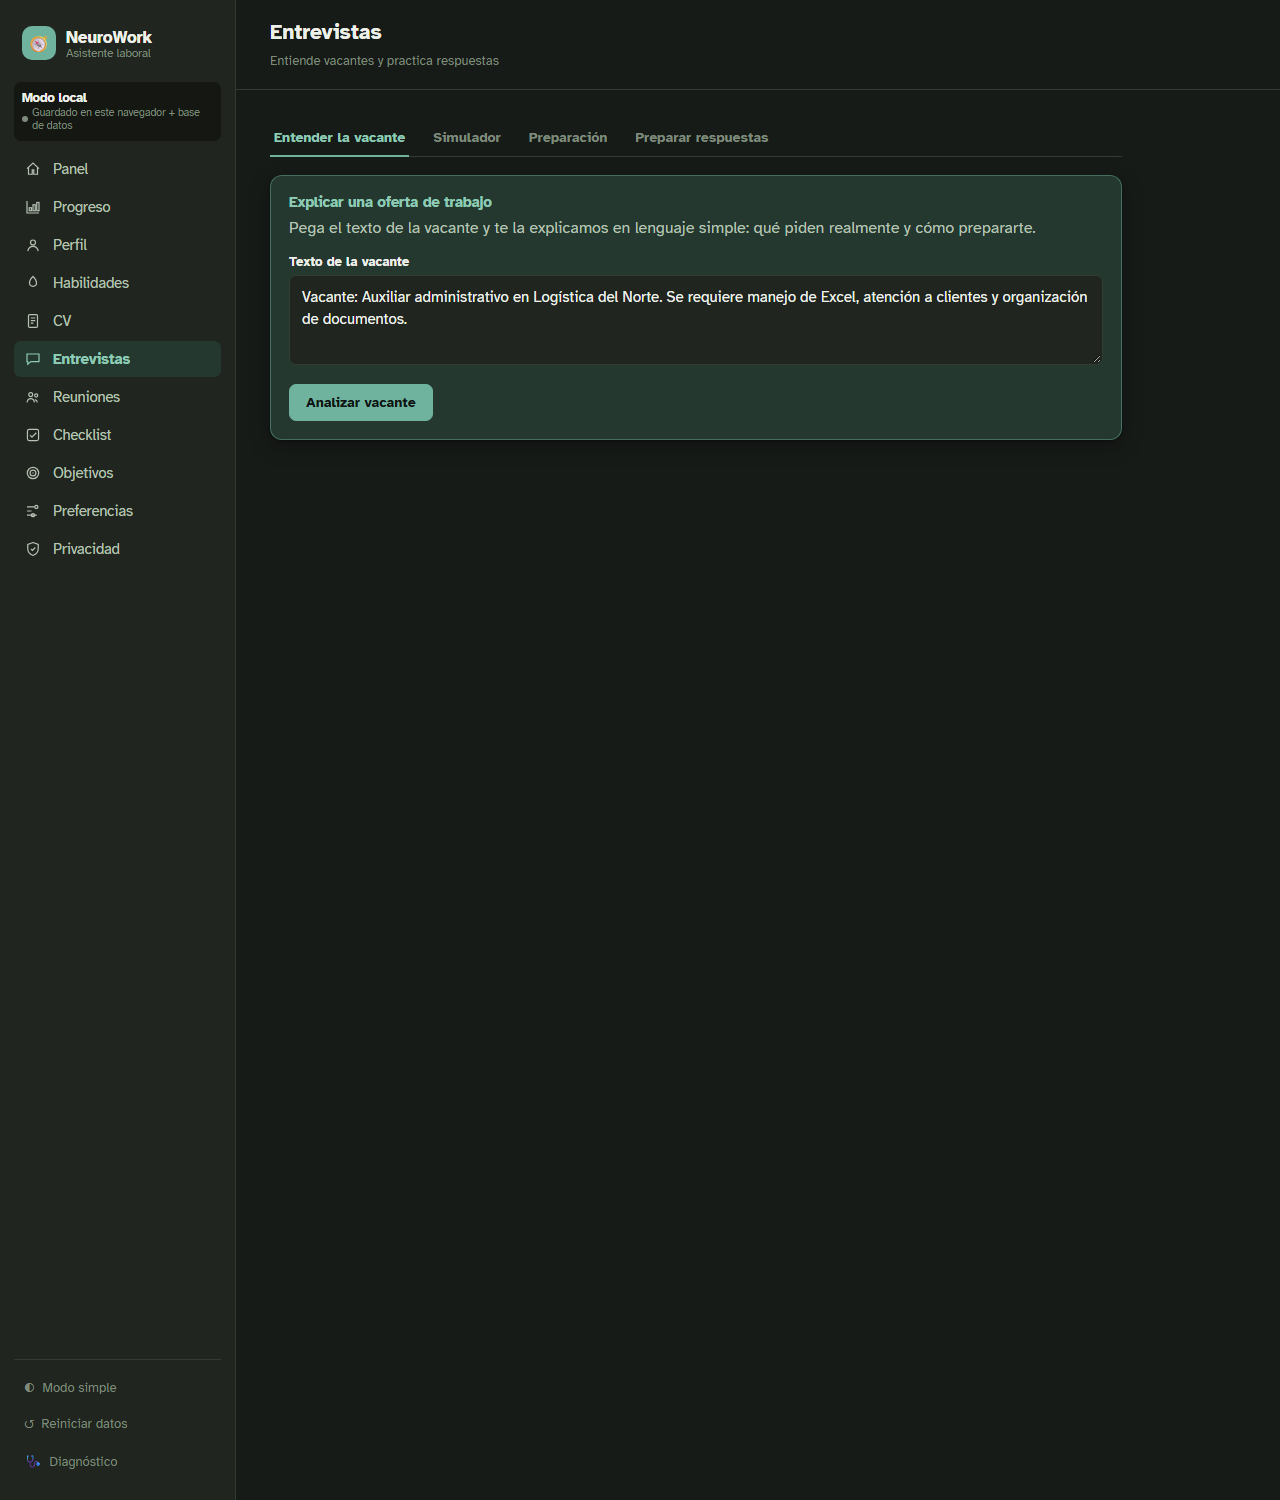
\includegraphics[width=\linewidth]{06-entrevistas.png}\end{minipage}\hfill
\begin{minipage}{0.49\textwidth}\centering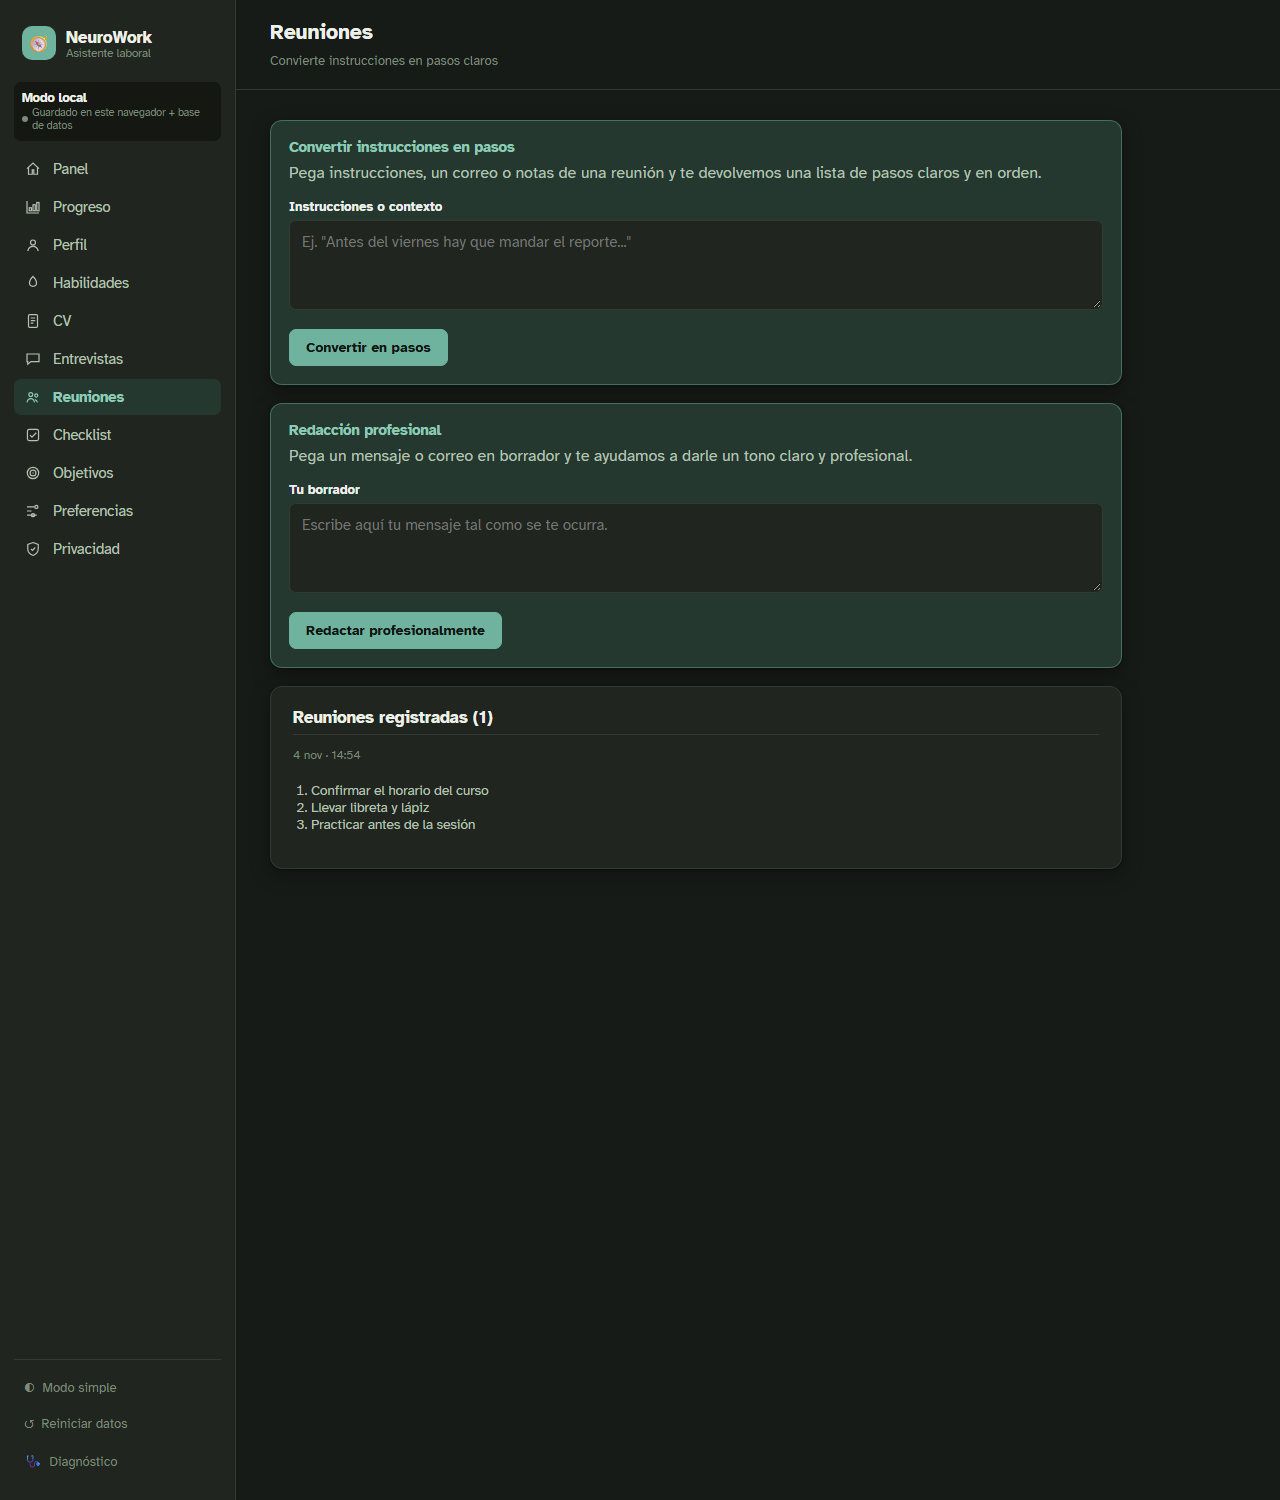
\includegraphics[width=\linewidth]{07-reuniones.png}\end{minipage}
\caption{Izquierda: entrevistas (cuatro pestañas). Derecha: reuniones convertidas en pasos.}
\end{figure}

\begin{figure}[htbp]
\centering
\begin{minipage}{0.49\textwidth}\centering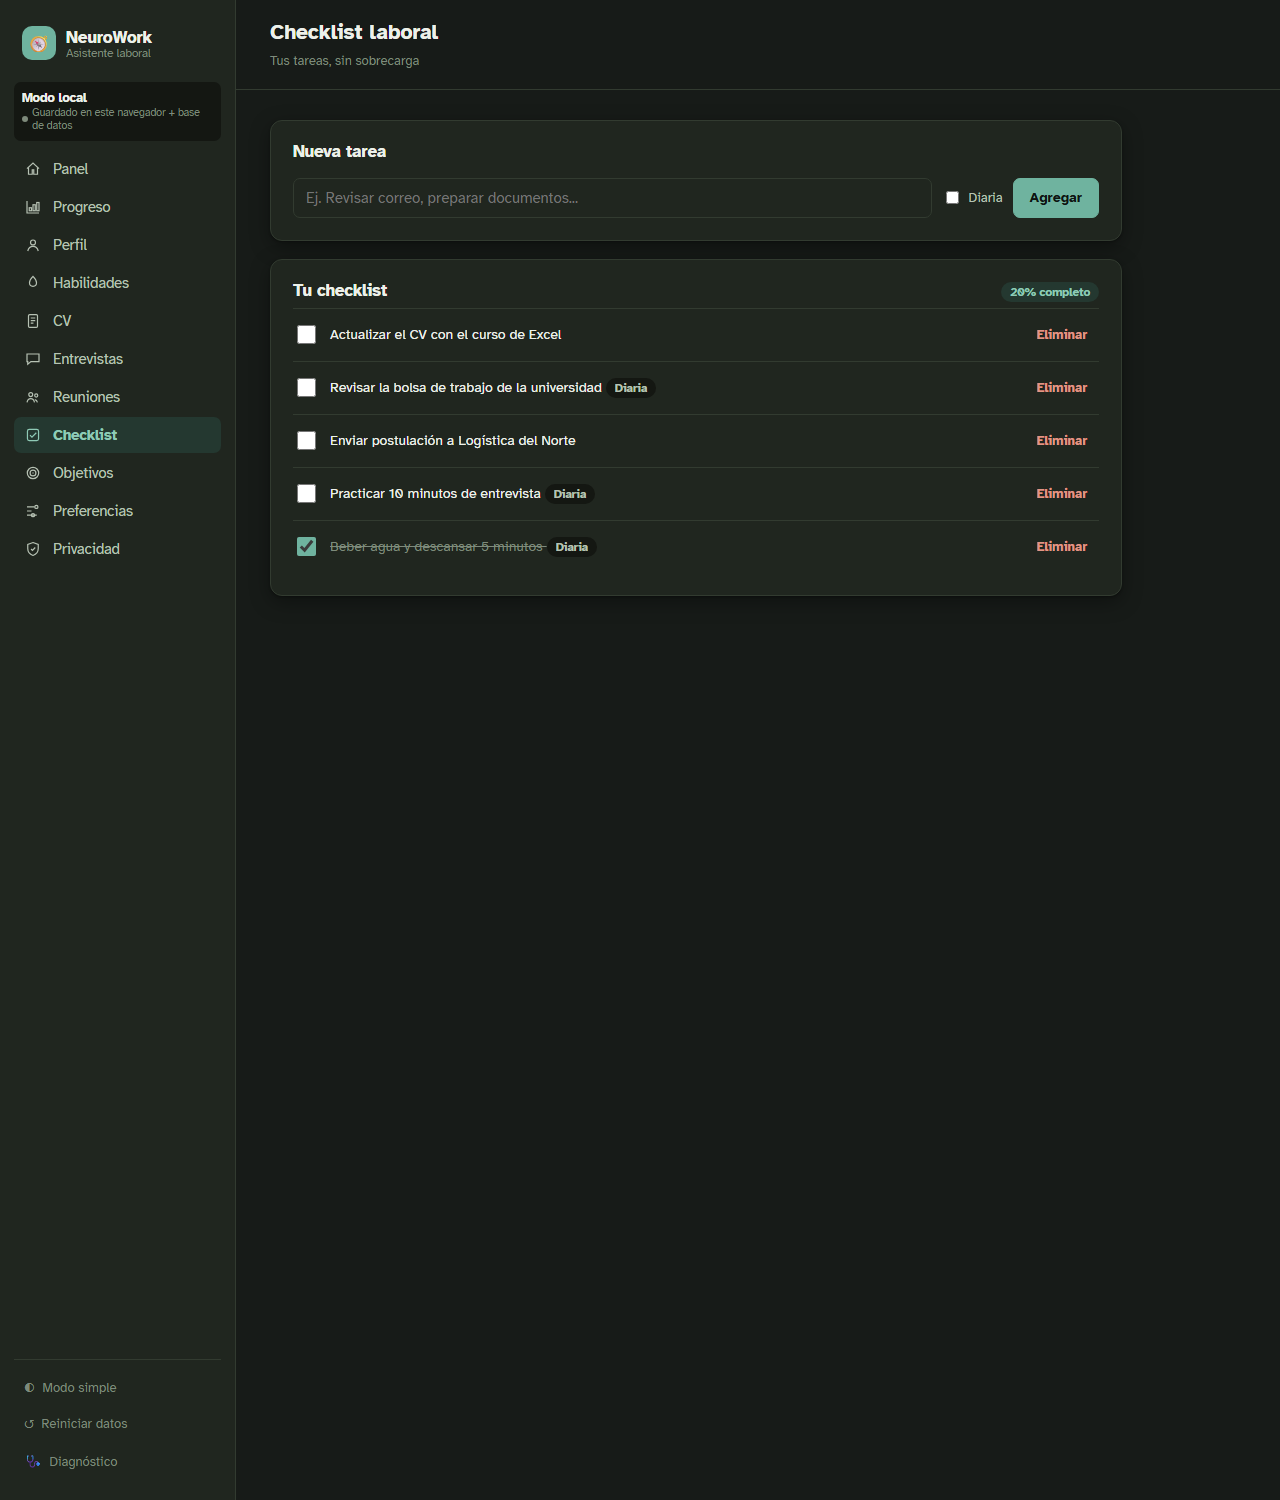
\includegraphics[width=\linewidth]{08-checklist.png}\end{minipage}\hfill
\begin{minipage}{0.49\textwidth}\centering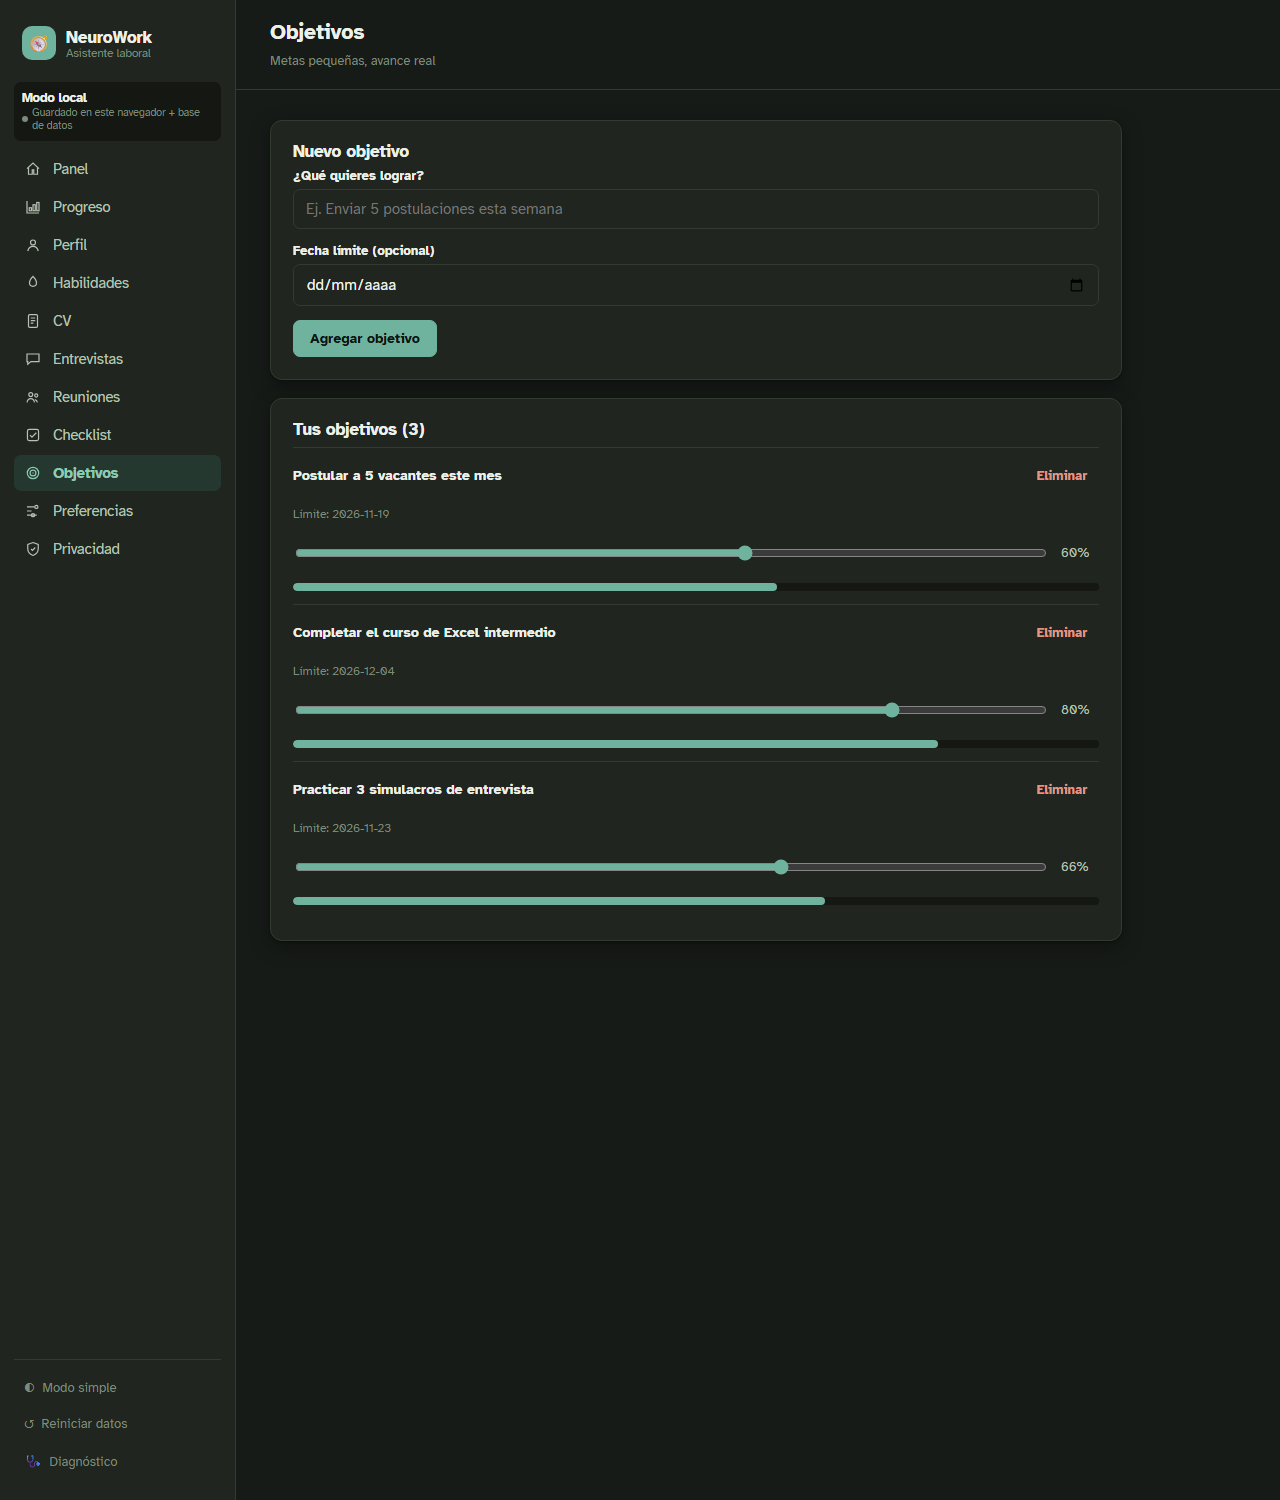
\includegraphics[width=\linewidth]{09-objetivos.png}\end{minipage}
\caption{Izquierda: checklist de tareas. Derecha: objetivos con fecha y porcentaje de avance.}
\end{figure}

\begin{figure}[htbp]
\centering
\begin{minipage}{0.49\textwidth}\centering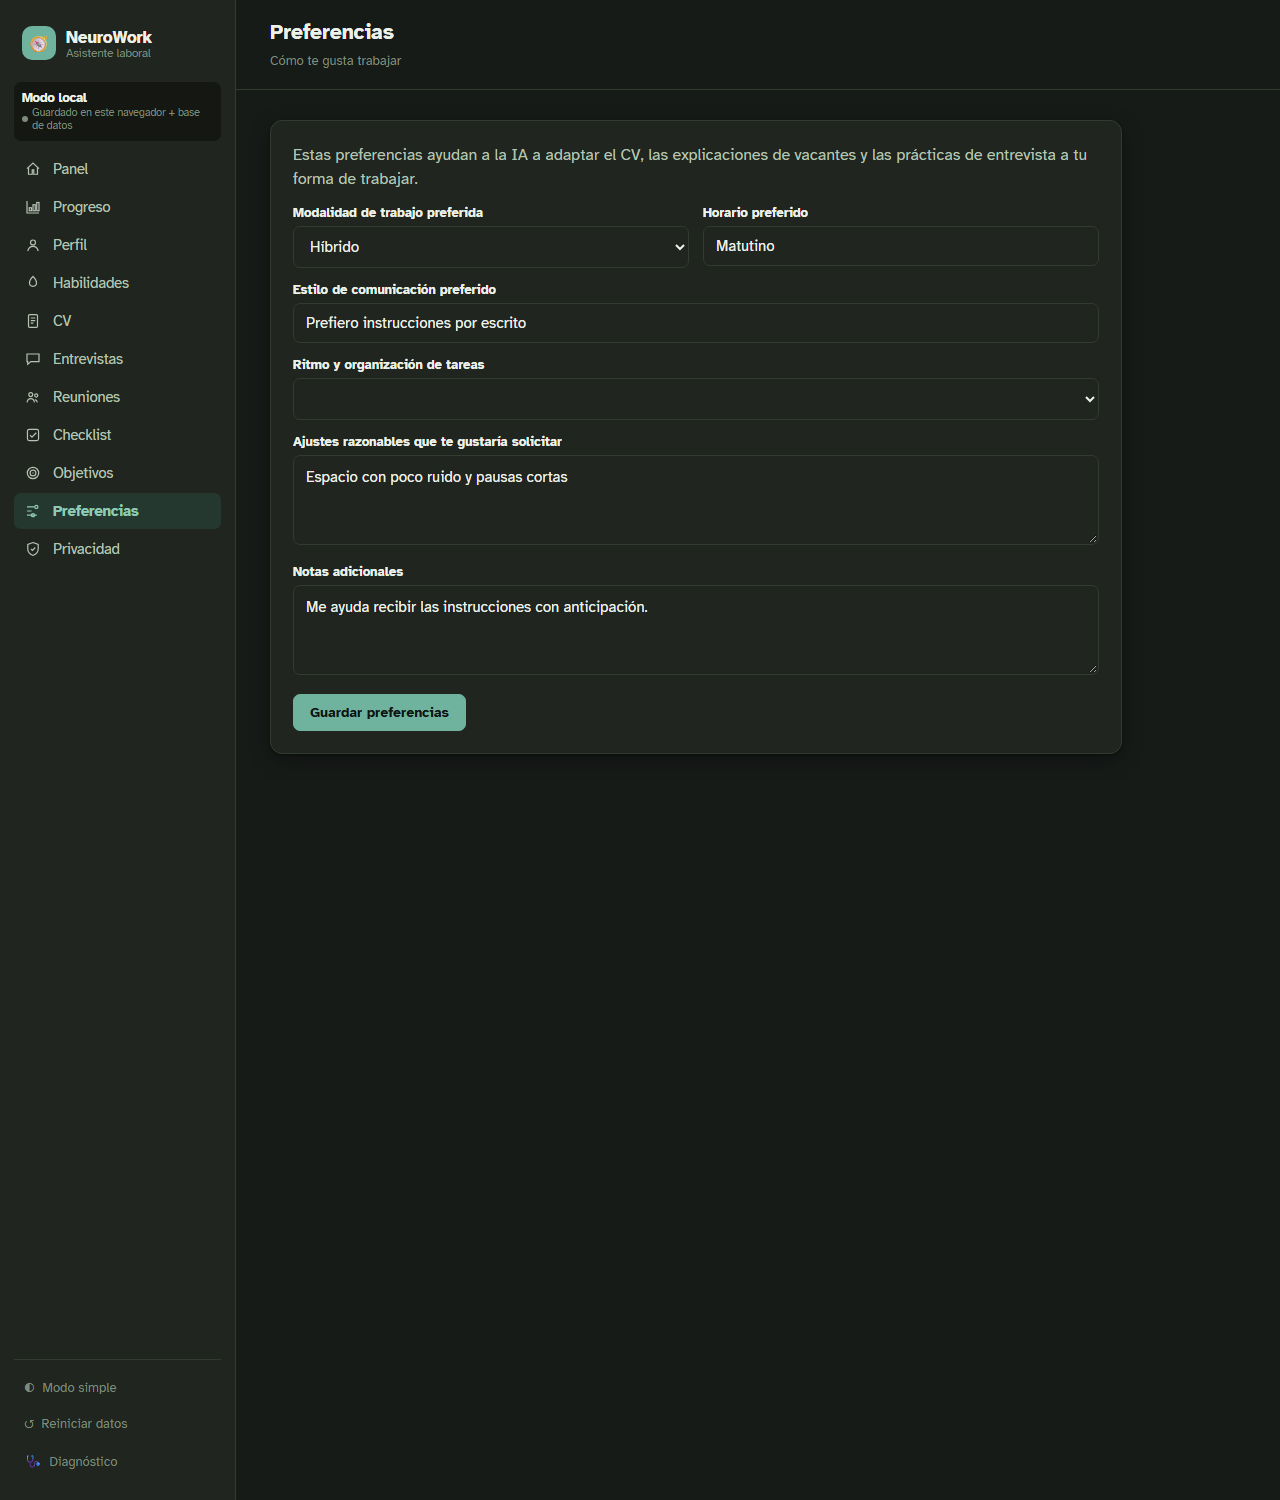
\includegraphics[width=\linewidth]{10-preferencias.png}\end{minipage}\hfill
\begin{minipage}{0.49\textwidth}\centering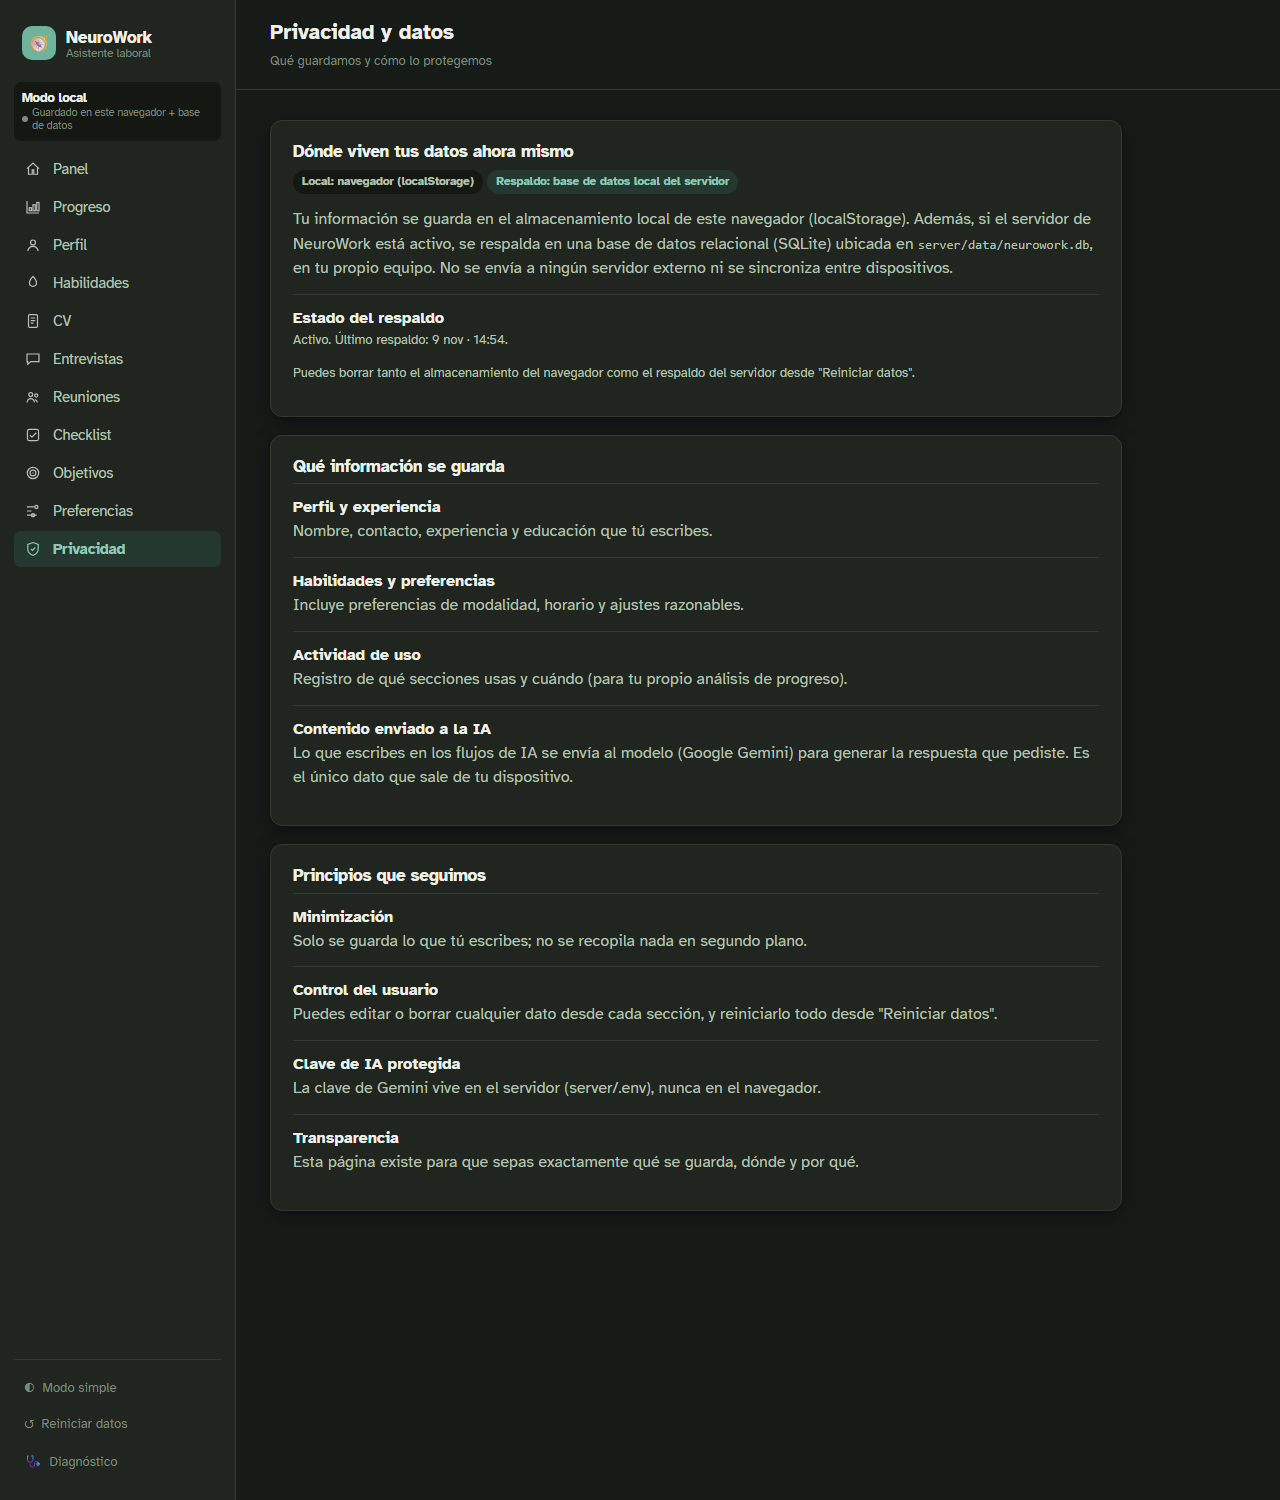
\includegraphics[width=\linewidth]{11-privacidad.png}\end{minipage}
\caption{Izquierda: preferencias de trabajo. Derecha: privacidad y estado del respaldo en la base de datos.}
\end{figure}

\begin{figure}[htbp]
\centering
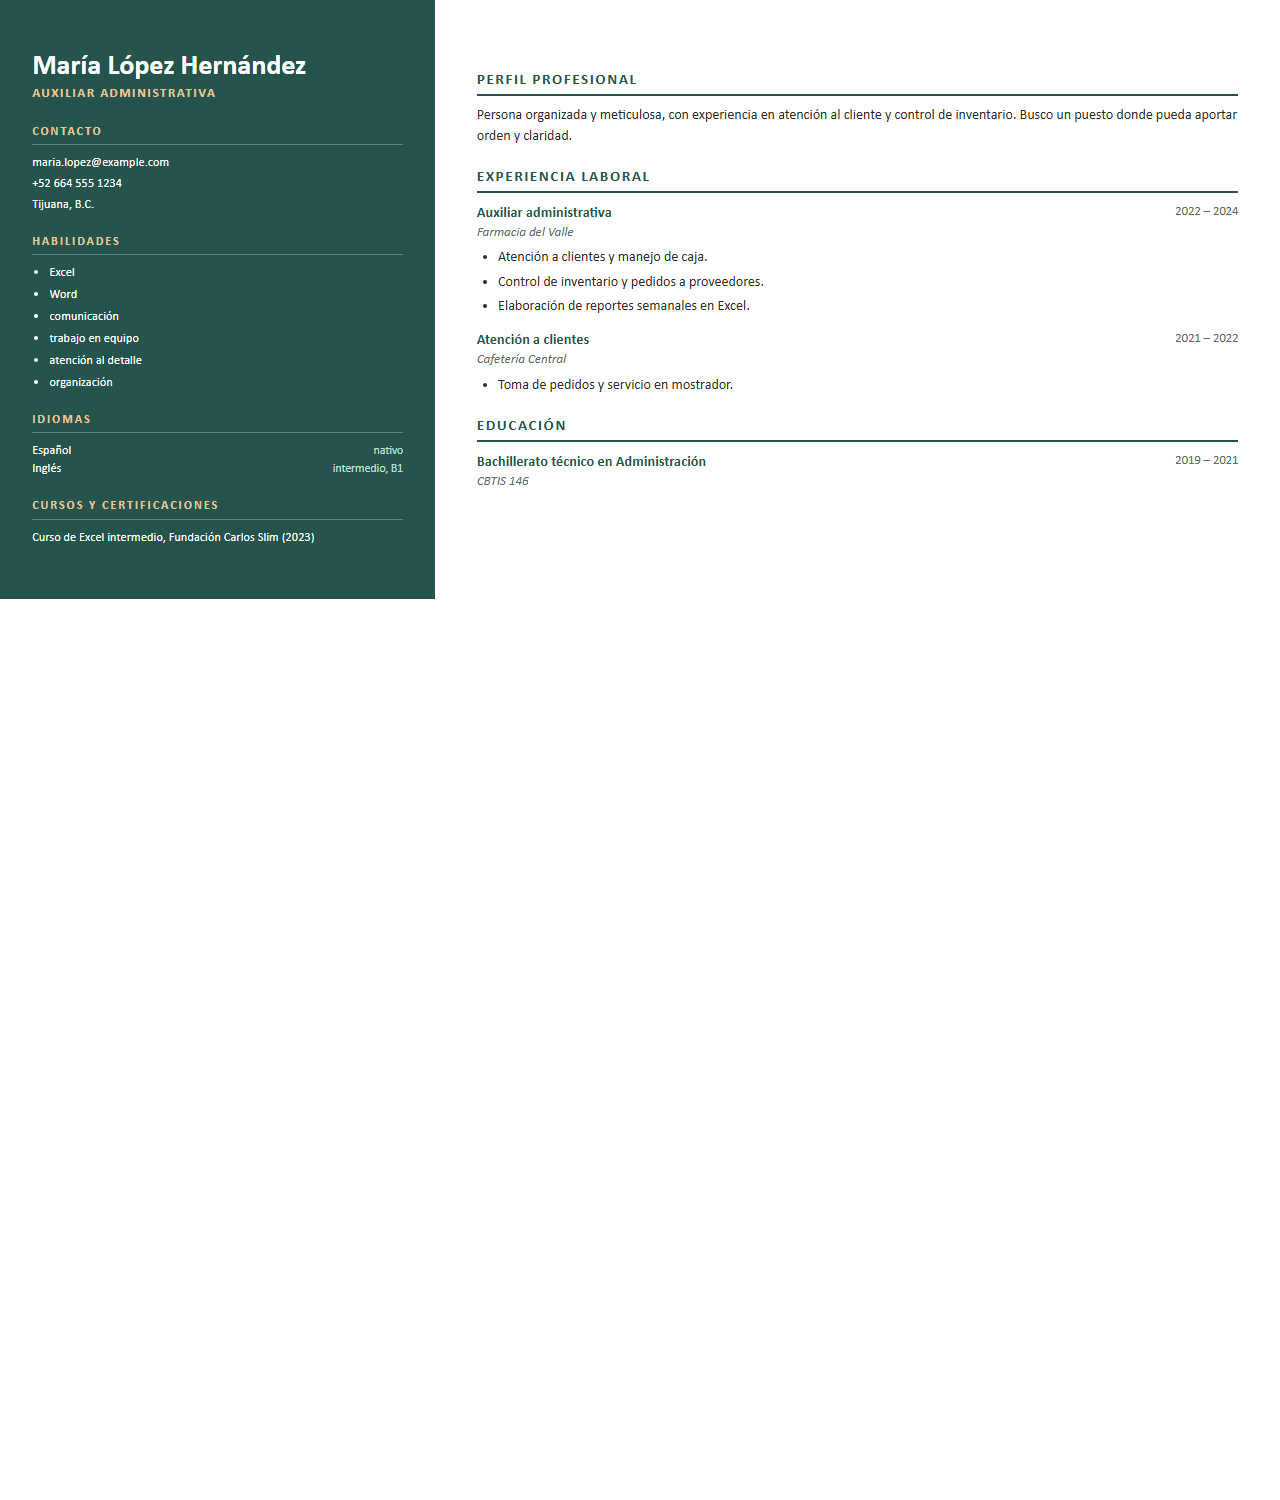
\includegraphics[width=0.86\textwidth]{12-cv-moderno.png}
\caption{Diseño de CV «Moderno»: dos columnas con barra lateral.}
\end{figure}

\begin{figure}[htbp]
\centering
\begin{minipage}{0.49\textwidth}\centering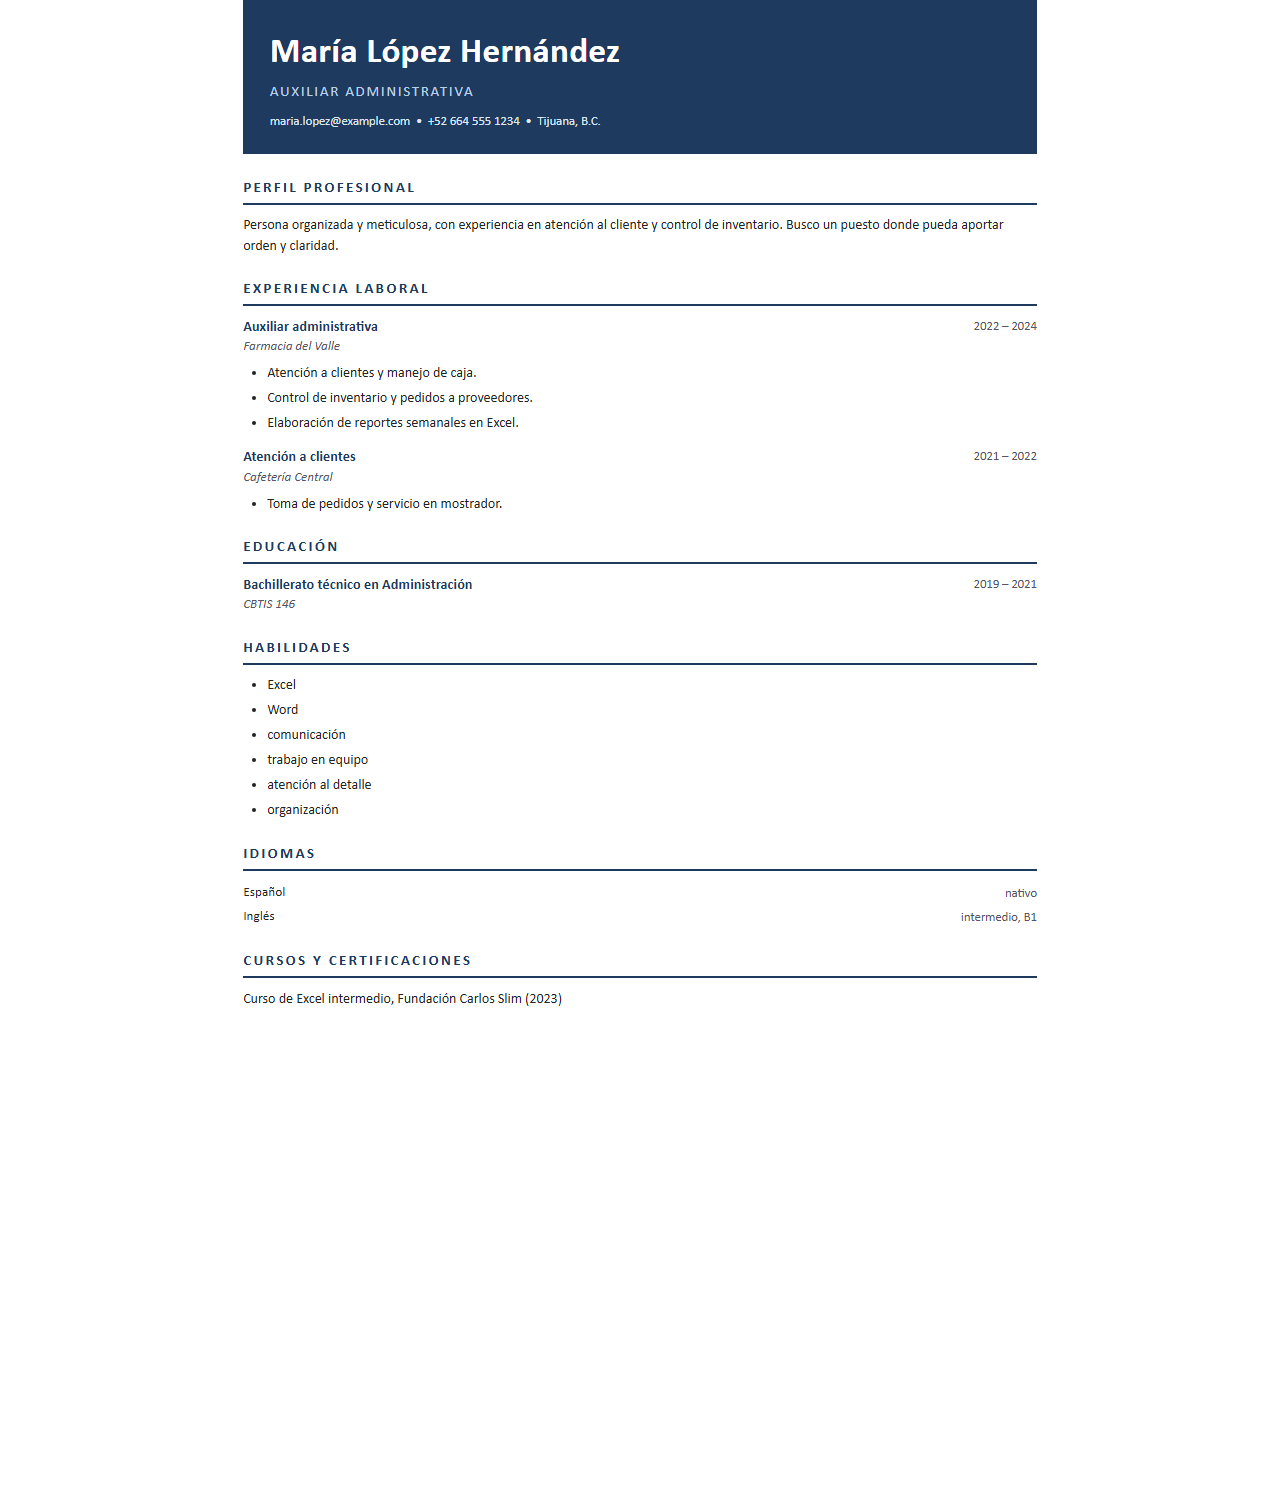
\includegraphics[width=\linewidth]{13-cv-ejecutivo.png}\end{minipage}\hfill
\begin{minipage}{0.49\textwidth}\centering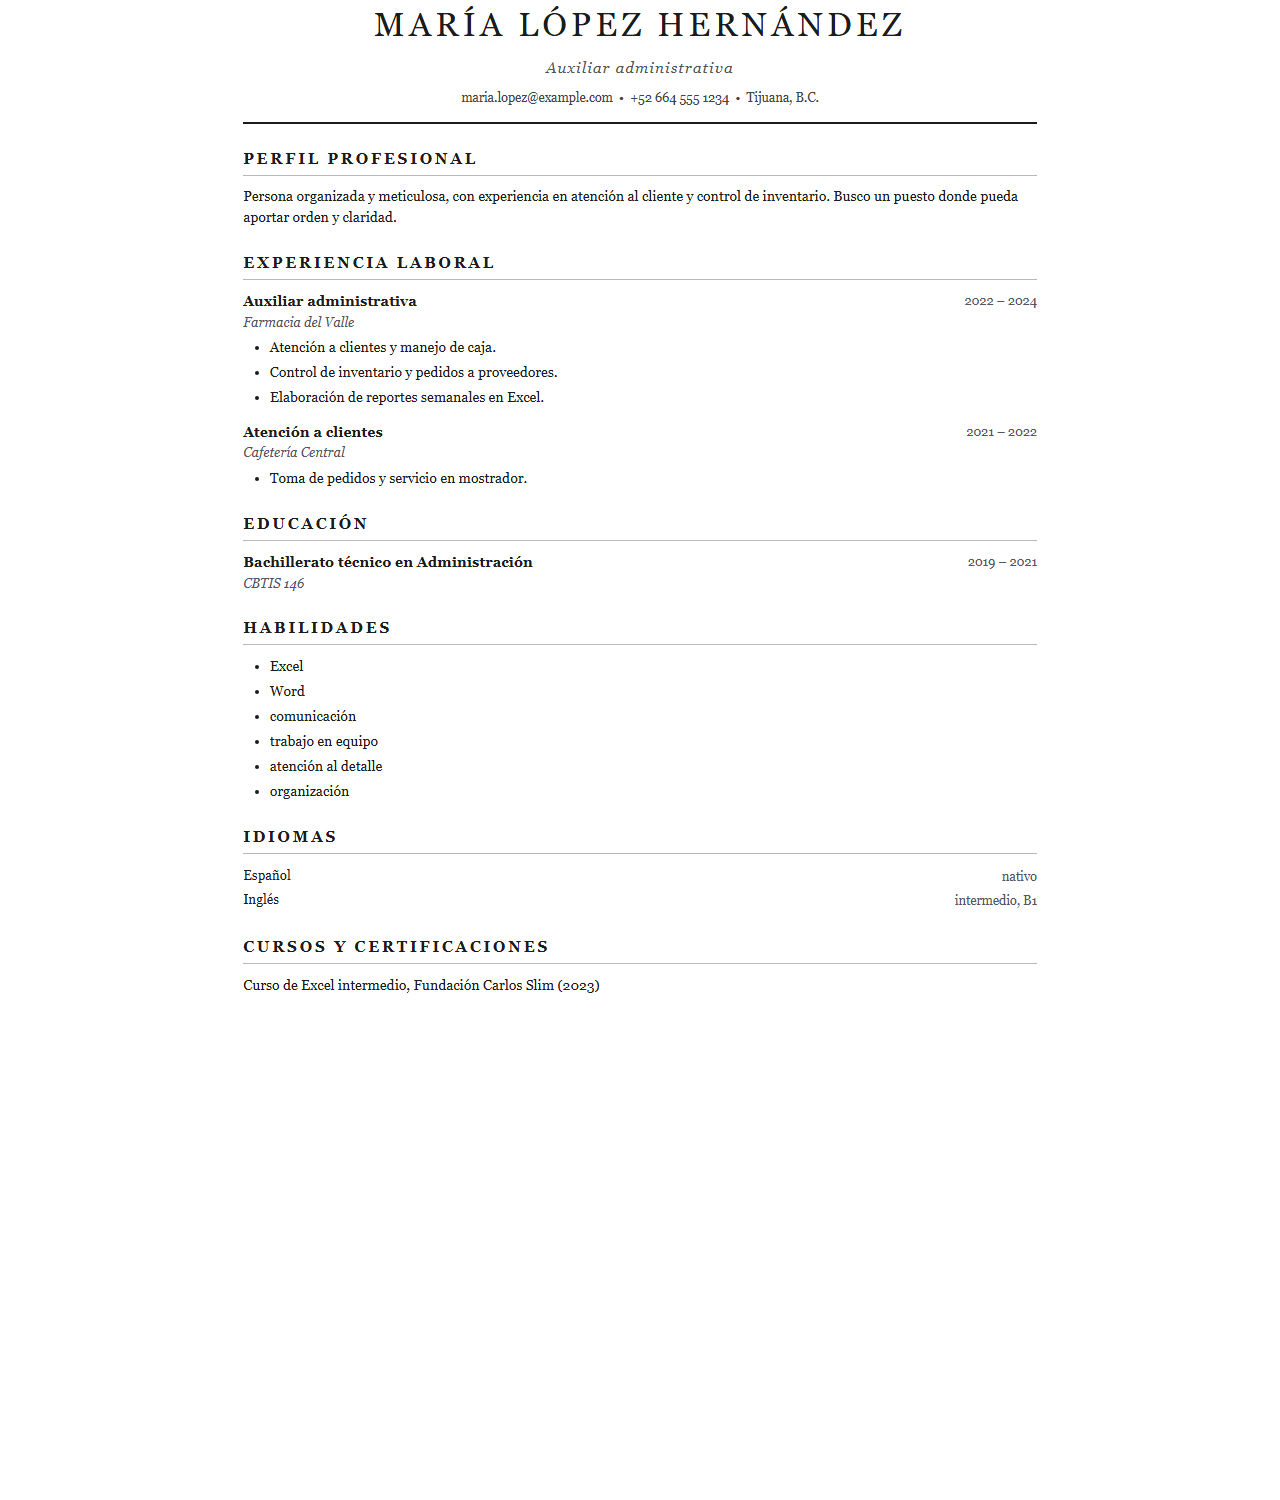
\includegraphics[width=\linewidth]{14-cv-clasico.png}\end{minipage}
\caption{Izquierda: diseño «Ejecutivo». Derecha: diseño «Clásico».}
\end{figure}

\begin{figure}[htbp]
\centering
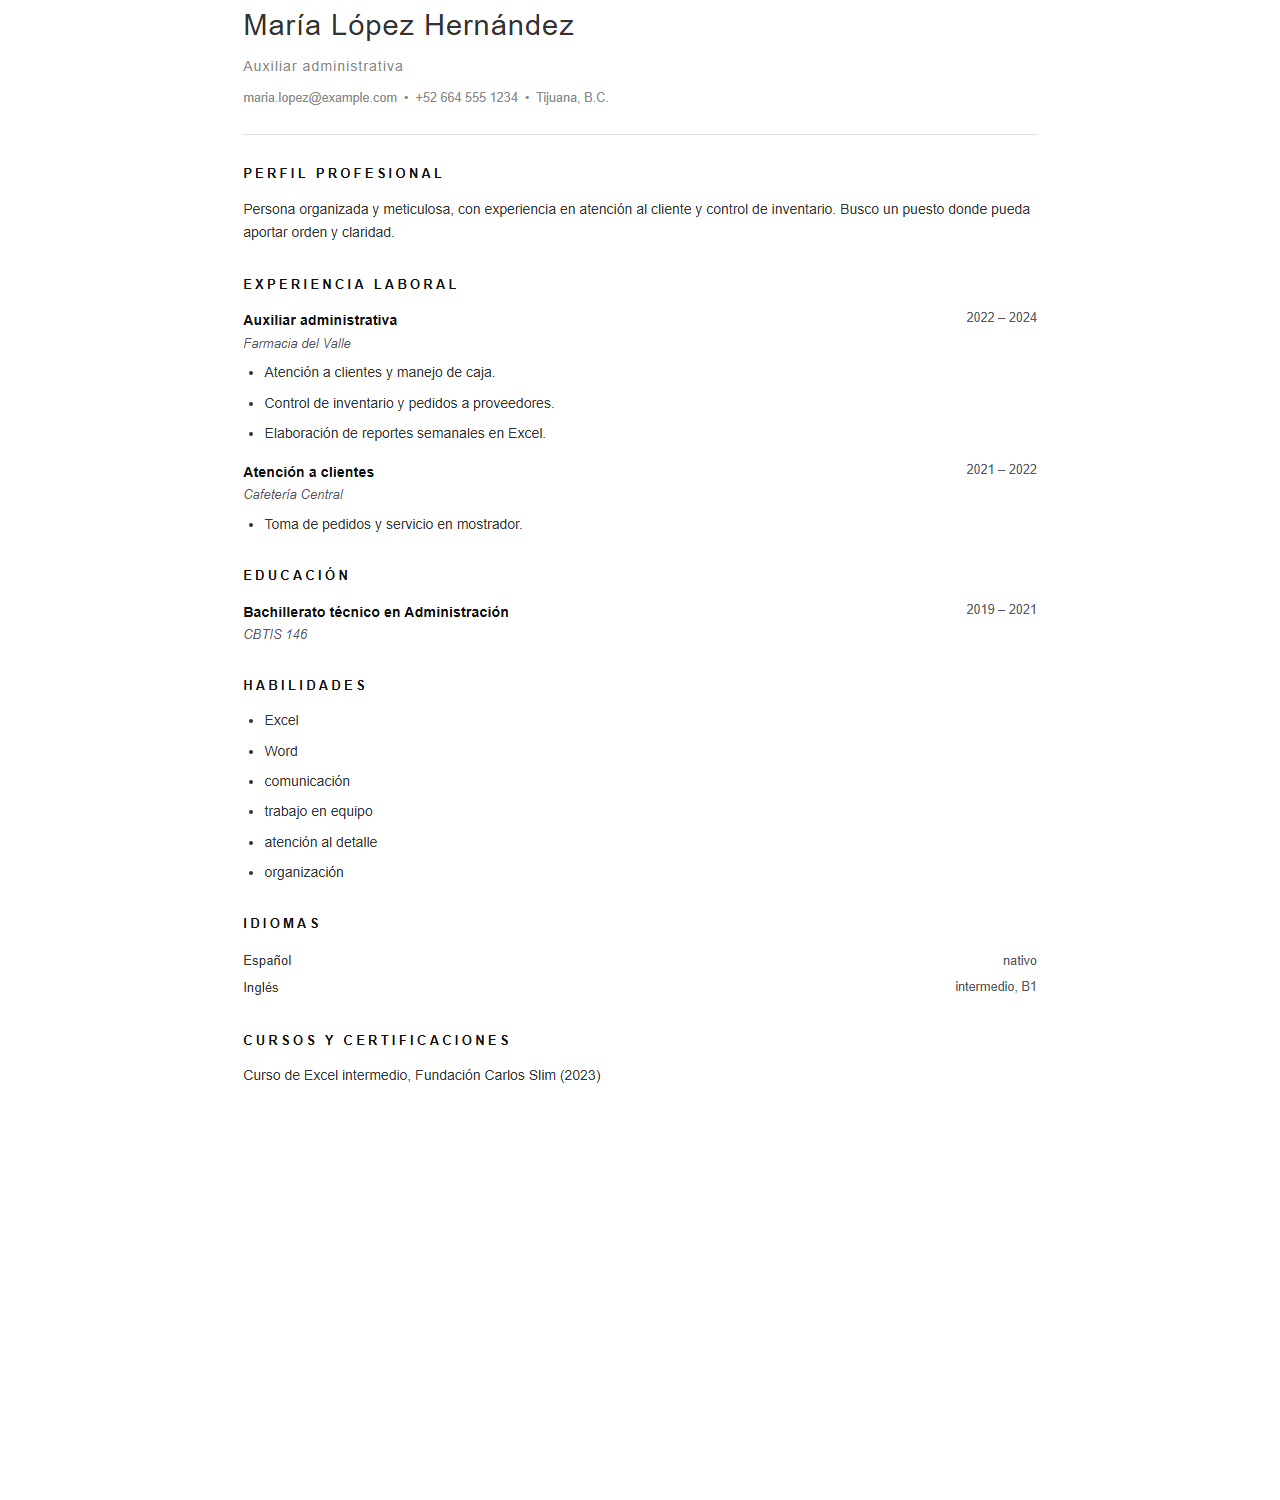
\includegraphics[width=0.86\textwidth]{15-cv-minimalista.png}
\caption{Diseño «Minimalista»: limpio y con amplio espacio en blanco.}
\end{figure}

\section{Comparación con el cronograma inicial}
El avance respecto al plan se resume en la Tabla~\ref{tab:cronograma}.

\begin{table}[htbp]
\caption{Comparación con el cronograma inicial.}
\label{tab:cronograma}
\centering
\small
\begin{tabular}{lll}
\toprule
Actividad planificada & Estado & Evidencia\\
\midrule
Anteproyecto y requerimientos & Completado & Descripción general (\texttt{docs/01}), anteproyecto\\
Arquitectura y modelo de datos & Completado & Arquitectura (\texttt{docs/03}), Base de datos (\texttt{docs/13})\\
Interfaz accesible & Completado & Accesibilidad (\texttt{docs/12}), \texttt{styles.css}\\
Módulos funcionales (11) & Completado & \texttt{app.js}\\
Integración de IA generativa & Completado (técnica) & \texttt{ai.js}, \texttt{server.js}\\
Base de datos relacional & Parcial (local) & \texttt{server/db.js}\\
Minería de datos & Completado & Minería de datos (\texttt{docs/06}), \texttt{analytics.js}\\
Capacidades PWA / offline & Completado & PWA (\texttt{docs/08}), \texttt{sw.js}\\
Pruebas técnicas & Completado & \texttt{tests/} (41)\\
Documentación técnica & En curso & \texttt{docs/01}--\texttt{15}\\
Validación con usuarios & Pendiente & fase final\\
\bottomrule
\end{tabular}
\end{table}

\textbf{Avance global estimado: $\sim$85\,\%.} Se consolidaron las actividades técnicas;
falta la validación empírica con usuarios y la exportación a PDF.

\section{Pruebas preliminares y validaciones}
\subsection{Pruebas automáticas}
Resultado: \textbf{41 pruebas, 41 correctas, 0 fallos} (Tabla~\ref{tab:pruebas}).

\begin{table}[htbp]
\caption{Distribución de las pruebas automáticas.}
\label{tab:pruebas}
\centering
\small
\begin{tabular}{lll}
\toprule
Archivo & Casos & Cubre\\
\midrule
\texttt{analytics.test.js} & 16 & Minería de datos y gráficas\\
\texttt{cv-doc.test.js} & 7 & Generación de documentos de CV\\
\texttt{db.test.js} & 7 & Base de datos (ida y vuelta, cascada)\\
\texttt{api.test.js} & 7 & API HTTP + base de datos (integración)\\
\texttt{server.test.js} & 4 & Seguridad y utilidades del servidor\\
\bottomrule
\end{tabular}
\end{table}

\subsection{Verificación manual y correcciones}
Verificación sintáctica con \texttt{node --check}; \texttt{/api/health} operativo;
comprobación en vivo de \texttt{PUT/GET/DELETE /api/state} y \texttt{GET /api/db} (23
tablas). Correcciones aplicadas: error \texttt{Failed to fetch} al abrir la app como archivo
(resuelto sirviendo por HTTP), incremento de la versión de caché del \emph{Service Worker},
rediseño del generador de CV (cuatro plantillas, fechas alineadas) y UTF-8 en los documentos
\texttt{.doc}.

\subsection{Retroalimentación}
\textbf{Aún no se ha realizado validación con usuarios finales.} No se reportan opiniones ni
resultados que no se hayan recogido formalmente. La prueba piloto con 2--3 personas
neurodivergentes está planificada para la fase final.

\section{Documentación técnica}
Diagrama de arquitectura y flujo: Arquitectura del sistema
(\texttt{docs/03-arquitectura.md}) y Base de datos (\texttt{docs/13-base-de-datos.md}).
Especificación de módulos: Módulos funcionales (\texttt{docs/04-modulos-funcionales.md}).
Flujos de IA: (\texttt{docs/05-flujos-de-ia.md}). Minería de datos:
(\texttt{docs/06-mineria-de-datos.md}). Seguridad: (\texttt{docs/07-seguridad.md}).
Base de datos: (\texttt{docs/13-base-de-datos.md}); ER, tablas, endpoints y mapeo.
Manual de usuario inicial: (\texttt{docs/14-manual-usuario.md}). Plan de cierre:
(\texttt{docs/15-plan-fase-final.md}).

\section{Plan de trabajo para la fase final}
\begin{table}[htbp]
\caption{Plan de trabajo para la fase final.}
\label{tab:plan}
\centering
\small
\begin{tabular}{clll}
\toprule
\# & Actividad pendiente & Entregable & Tiempo\\
\midrule
1 & Validación con usuarios (2--3) & Informe de usabilidad & 4--5 días\\
2 & Exportación del CV a PDF & Botón «Descargar PDF» & 2--3 días\\
3 & Migración y respaldo de la BD & Script de migración & 2 días\\
4 & Pruebas E2E completas & Checklist con evidencias & 2 días\\
5 & Accesibilidad (WCAG 2.2 AA) & Informe de conformidad & 2--3 días\\
6 & Refinamiento UI/UX & Ajustes documentados & 3 días\\
7 & Documentación final y memoria & Memoria + diagramas & 4--5 días\\
8 & Presentación y demo & Diapositivas + video & 2 días\\
\bottomrule
\end{tabular}
\end{table}

\noindent\textbf{Recursos:} desarrollo individual, asesoría del profesor y usuarios
voluntarios. \textbf{Tiempo total estimado:} $\sim$4 semanas. \textbf{Entregables
planeados:} prototipo completo, base de datos con migración, suite de pruebas en verde,
memoria técnica, manual de usuario y evidencias (repositorio, capturas, video).

\end{document}
